%==============================================================================
% Figure: Cayley-Dickson Tree Diagram
% Purpose: Visual representation of dimensional doubling construction
% Chapter: Ch02 - Cayley-Dickson Algebras
% Type: Tree diagram / Hierarchy visualization
%==============================================================================

\begin{figure}[htbp]
  \centering
  \resizebox{\textwidth}{!}{%
  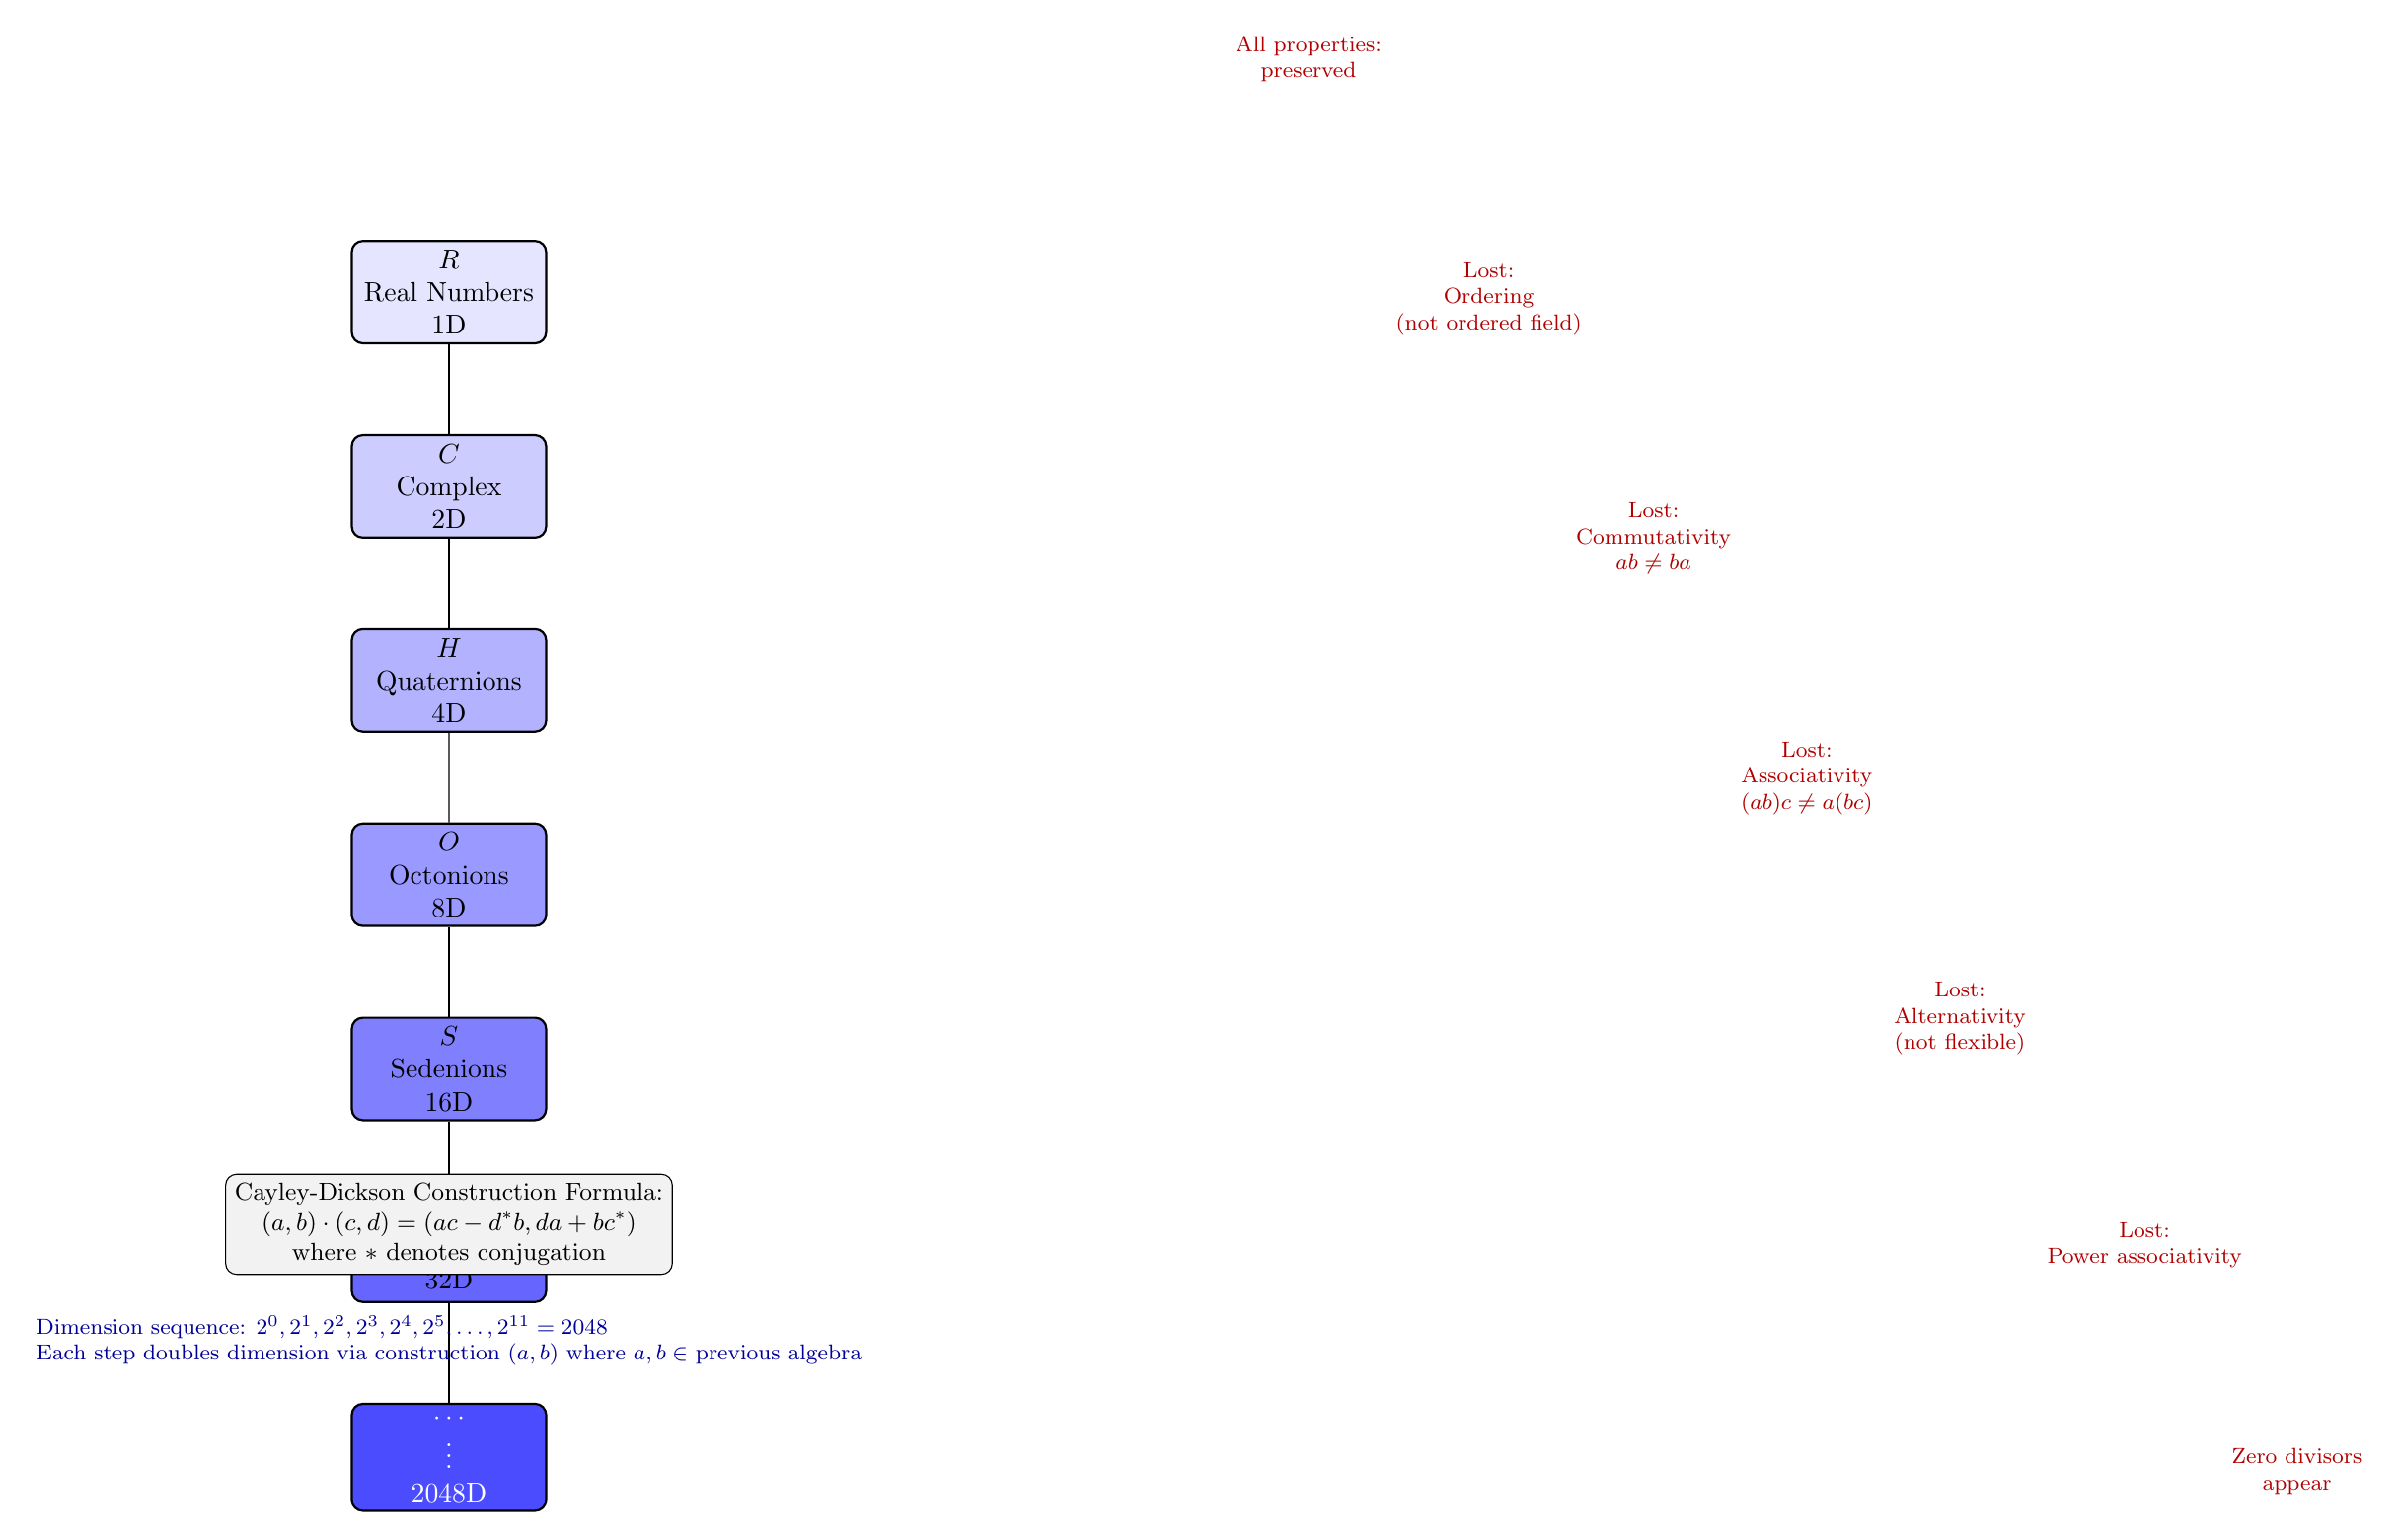
\begin{tikzpicture}[
    level distance=2.5cm,
    level 1/.style={sibling distance=8cm},
    level 2/.style={sibling distance=4cm},
    level 3/.style={sibling distance=2cm},
    algebra/.style={
      rectangle,
      rounded corners,
      minimum width=2.5cm,
      minimum height=1cm,
      text centered,
      align=center,
      draw=black,
      line width=0.8pt,
      font=\normalsize
    },
    arrow/.style={
      thick,
      ->,
      >=stealth,
      line width=1pt
    },
    property/.style={
      font=\footnotesize,
      text=red!70!black,
      align=center
    }
  ]

    % Root: Real numbers
    \node[algebra, fill=blue!10] {$\mathbb{R}$\\Real Numbers\\1D}
      child {
        node[algebra, fill=blue!20] {$\mathbb{C}$\\Complex\\2D}
        child {
          node[algebra, fill=blue!30] {$\mathbb{H}$\\Quaternions\\4D}
          child {
            node[algebra, fill=blue!40] {$\mathbb{O}$\\Octonions\\8D}
            child[grow=south] {
              node[algebra, fill=blue!50] {$\mathbb{S}$\\Sedenions\\16D}
              child[grow=south] {
                node[algebra, fill=blue!60] {Pathions\\32D}
                child[grow=south] {
                  node[algebra, fill=blue!70, text=white] {$\cdots$\\$\vdots$\\2048D}
                }
              }
            }
          }
        }
      };

    % Property annotations - positioned to the right of each level
    \node[property, anchor=west, xshift=10cm, yshift=3cm]
      (prop1) {All properties:\\preserved};

    \node[property, right of=prop1, anchor=north west, yshift=-2.5cm]
      (prop2) {Lost:\\Ordering\\(not ordered field)};

    \node[property, right of=prop2, anchor=north west, yshift=-2.5cm]
      (prop3) {Lost:\\Commutativity\\$ab \neq ba$};

    \node[property, right of=prop3, anchor=north west, yshift=-2.5cm]
      (prop4) {Lost:\\Associativity\\$(ab)c \neq a(bc)$};

    \node[property, right of=prop4, anchor=north west, yshift=-2.5cm]
      (prop5) {Lost:\\Alternativity\\(not flexible)};

    \node[property, right of=prop5, anchor=north west, yshift=-2.5cm]
      (prop6) {Lost:\\Power associativity};

    \node[property, right of=prop6, anchor=north west, yshift=-2.5cm]
      (prop7) {Zero divisors\\appear};

    % Construction formula at bottom
    \node[
      draw,
      rounded corners,
      fill=gray!10,
      font=\small,
      align=center,
      yshift=-12cm
    ] (formula) {
      Cayley-Dickson Construction Formula:\\
      $(a, b) \cdot (c, d) = (ac - d^*b, da + bc^*)$\\
      where $*$ denotes conjugation
    };

    % Dimension count annotation
    \node[
      font=\footnotesize,
      text=blue!60!black,
      align=left,
      below of=formula,
      yshift=-0.5cm
    ] {
      Dimension sequence: $2^0, 2^1, 2^2, 2^3, 2^4, 2^5, \ldots, 2^{11} = 2048$\\
      Each step doubles dimension via construction $(a,b)$ where $a,b \in$ previous algebra
    };

  \end{tikzpicture}%
  }

  \caption{Cayley-Dickson tree showing the doubling construction from real numbers ($\mathbb{R}$, 1D) to 2048-dimensional algebra. Each level doubles the dimension but loses a fundamental algebraic property (indicated in red). The construction continues indefinitely, but physical frameworks typically use 2--16D (complex through sedenions) or higher powers of 2. This structure provides the dimensional hierarchy underlying multi-dimensional field theories in the Aether framework.}
  \label{fig:cayley-dickson-tree}
\end{figure}
